\chapter{Resources and Interactivity}

\section{Introduction}
...To be filled...

\section{Android Resources}
A decent android application typically contains many different kinds of assets. It can display images on the screen, play videos, render text, play animations and sounds etc. Assets are an integral part of any mobile app. Usually the artists generate assets and programmers write source code for logic and to present these assets to the user in an effective manner.

In android development assets are referred to as ``Resources''. Almost everything is a ``resource''. A layout is a resource, string table is a resource, an image is a resource. You can include custom resources in your project even if the type and format is unknown to android studio. More information about resources can be found at:

\url{https://developer.android.com/guide/topics/resources/overview.html}

Android studio places all the resources related to each project inside a very special directory called ``\texttt{res}''. Similarly it places all of the source code in a directory called ``\texttt{java}''. Let's explore different types of resources.

\subsection{Create new project}
\label{RAI:createProj}

Create a new project from scratch. Perform the following steps:
\begin{enumerate}
	\item Create a new project having name ``\texttt{Lec4}''
	\item Select minimum API 16 : Android 4.1 (Jelly Bean).
	\item Select ``\texttt{Empty Activity}''
	\item Accept default values for activity and click finish. \\
\end{enumerate}

Once the project is created, go to the panel on the left side, also called the ``project panel''. Make sure that the ``Project'' view is selected from the drop down menu at the top. This view shows the actual physical directory structure of the project as it exists on the hard disk. You can expand any directory by clicking on the little arrow icon present at its left side. \\

All of the project source code and resources are located inside the \texttt{main} folder:

\texttt{Lec4} $\rightarrow$ \texttt{app} $\rightarrow$ \texttt{src} $\rightarrow$ \underline{\textbf{\texttt{main}}}

\begin{center}
	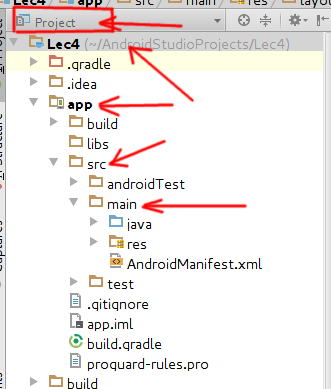
\includegraphics[scale=0.4]{chapters/ch04/images/1_project_panel}
\end{center}

The \texttt{main} folder contains two sub-folders and a very important xml file called ``AndroidManifest.xml'' (this file contains very important app related settings and configurations. We will talk about in detail in future). 

The \texttt{$\backslash$java} folder contains all of the project related source code. The directory structure is similar to the standard java package convention. Try exploring it and see what kind of code is inside it.

The \texttt{$\backslash$res} folder contains all of the project related resources. Sound files, music, images, movies, layout xml, or any custom asset will go into this directory. \\

Let's explore the \texttt{$\backslash$res} a little bit more and see what's inside it. Click and expand \texttt{res}. 

\begin{center}
	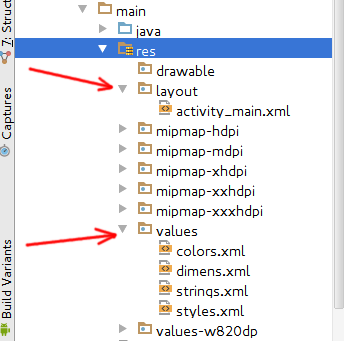
\includegraphics[scale=0.4]{chapters/ch04/images/2_res_folder}
\end{center}

As you can see this folder contains a lot of other sub-folders. Each different sub-folder contains different types of resources. For example \texttt{layout} sub-folder contains the layouts for the app, \texttt{drawables} contains pictures and so on. Some sub-folders may have very similar names only differing in the suffix, such as \texttt{mipmap-mdpi}, \texttt{mipmap-hdpi}, \texttt{mipmap-xdpi} etc. These usually contain same types of resources. We will look into it in detail later on. \\

For the time being the two folders we are interested in are the \texttt{layout} and \texttt{values}. As already mentioned ``\texttt{layout}'' contains layout xml files that describes the physical appearance of the activities. ``\texttt{values}'' contains a set of strings (and other types of measurements) that your app will use. \\

For more information on other types of resources please visit \href{https://developer.android.com/guide/topics/resources/available-resources.html}{here}.

\subsection{The String Resource}
Strings are used almost everywhere: on buttons, in labels, alongside radio buttons. There are essentially two categories of strings: 

\begin{enumerate}
	\item The ones used in source code. These are generally for internal system usage, the user can't see these.
	\item The ones that are actually displayed on the app screen. The user will see and interact with these types of strings.
\end{enumerate}

Let's see a practical example. Go to the project panel again. Make sure that ``Project'' mode is selected so that you can view actual physical directory structure. Inside the \texttt{values} folder you should see ``\texttt{strings.xml}'' file:

\begin{center}
	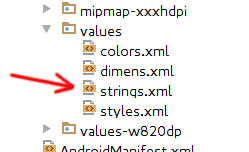
\includegraphics[scale=0.4]{chapters/ch04/images/3_strings}
\end{center}

Double click \texttt{strings.xml}, android studio will open it in the editor. This is a standard xml file format which contains strings to be used in our app (specially the layouts). All of the strings are defined inside \texttt{<resources>} tags:

\begin{center}
	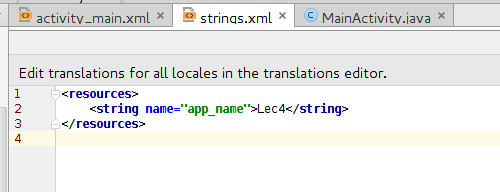
\includegraphics[scale=0.4]{chapters/ch04/images/4_strings_xml}
\end{center}

The actual strings are defined by the \texttt{<string>} tag. Right now there is only one string defined in our app, hence you see only one \texttt{<string>} tag. The name of the string is its ``\textbf{\texttt{id}}'' that you will refer to in your project java code or xml. The text in-between the string opening and closing tags is the actual string that you see on the screen (in this case ``Lec4'').

There are many ways to create new strings: manually, through translation editor or through layout text mode. You can use anyone you like.

\subsubsection{Creating strings manually}
Open up \texttt{strings.xml} in the editor window. Add a new string tag, give it a name ``\texttt{hello\_str}'' and text ``\texttt{Hello World !!!}'' (as done in line 3 below):

\begin{center}
	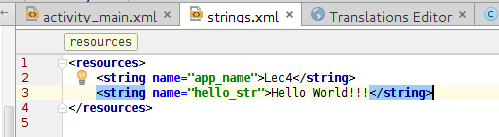
\includegraphics[scale=0.4]{chapters/ch04/images/5_new_string1}
\end{center}

\subsubsection{Creating strings through translation editor}
Open up any layout file, \texttt{activity\_main.xml} in our case. Go to the design mode, find an ``earth'' icon in the toolbar located at the top of the preview panel, select ``Edit Translations''.

\begin{center}
	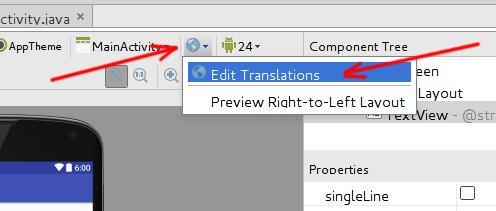
\includegraphics[scale=0.4]{chapters/ch04/images/9}
\end{center}

This will open up the translation editor. You can see the string that we created in the previous step. 

\begin{center}
	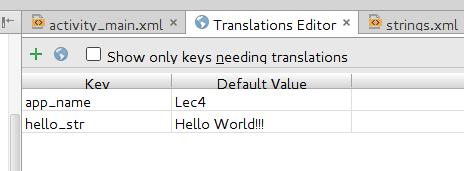
\includegraphics[scale=0.4]{chapters/ch04/images/11}
\end{center}

Click on the ``+'' button located at the upper left side of the editor. This will open up a small dialog box:

\begin{center}
	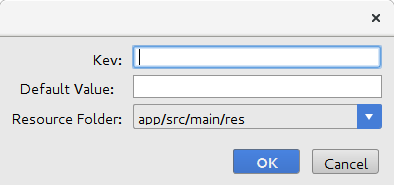
\includegraphics[scale=0.4]{chapters/ch04/images/10}
\end{center}

Enter ``\texttt{editor\_str}'' as the key (without quotes) and ``\texttt{This string was created from translation editor}'' as default value (again without quotes). Hit OK. The translator will update to show changes. If you open up \texttt{strings.xml} you will see the new string that we created from translation editor. \\

\textit{So basically the translation editor is just a front end interface for editing \texttt{strings.xml} !!!}

\subsubsection{Creating strings through layout text mode}
Open up ``\texttt{activity\_main.xml}'' and go to line 15. You can see the text of the view is hardcoded as ``Hello World!''. Bring your keyboard cursor onto the ``Hello World!'' string. A small yellow bulb icon will appear to its left side:

\begin{center}
	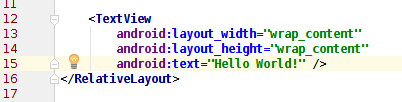
\includegraphics[scale=0.4]{chapters/ch04/images/12}
\end{center}

Using your mouse cursor click the bulb, this will bring a menu. Select ``Extract string resource'':

\begin{center}
	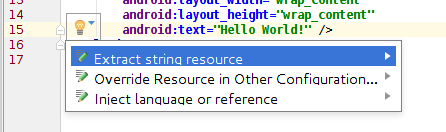
\includegraphics[scale=0.4]{chapters/ch04/images/13}
\end{center}

This will bring up a dialog box. Enter ``\texttt{new\_Lbl}'' as the ``Resource name''. Remember that string ``name'' is the id of that string resource:

\begin{center}
	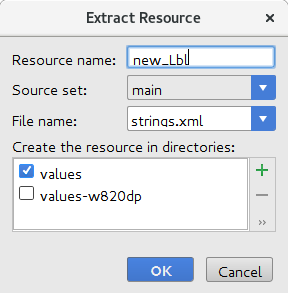
\includegraphics[scale=0.4]{chapters/ch04/images/14}
\end{center}

Accept all other values as default and press OK to dismiss the dialog. If you go to the ``\texttt{activity\_main.xml}'' file in text mode, notice that line 15 has now changed. The hardcoded string is replaced with the string resource id:

\begin{center}
	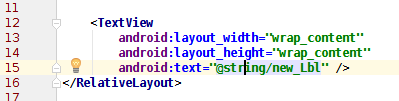
\includegraphics[scale=0.4]{chapters/ch04/images/15}
\end{center}

If you open up ``\texttt{strings.xml}'' you will see a new string created having name as \texttt{new\_Lbl}. \\

Ok go back to ``\texttt{activity\_main.xml}'' and set the text of the view back to the hardcoded ``\texttt{Hello World!}'' so that we can perform the next step!


\subsubsection{Using a string resource}

If not already then open up ``\texttt{activity\_main.xml}'' in text mode to view its xml source. The root layout (which happens to be \texttt{RelativeLayout}) has only one child: a text view (lines 12 to 15). Line 15 is hardcoding the string ``\texttt{Hello World!}'' as the text of the view.

\begin{center}
	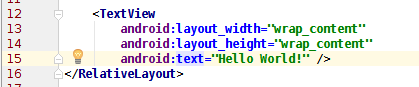
\includegraphics[scale=0.4]{chapters/ch04/images/6_new_string2}
\end{center}

Let's replace this hardcoded string with a string resource. Delete the string in line 15 and replace it with ``\texttt{@string/hello\_str}'' (including quotes):

\begin{center}
	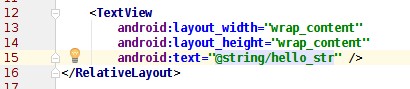
\includegraphics[scale=0.4]{chapters/ch04/images/7_new_string3}
\end{center}

The ``\texttt{@string/}'' part means that you are trying to access the string resource. (You can access any type of resource in the text mode by prefixing it with \texttt{@} symbol and then type of the recourse.) The second part is the \texttt{id} or \texttt{name} of the string that you want to use i.e: ``\texttt{hello\_str}''. We created this string earlier, now we are referring to that string resource in our layout file. As you are typing the android studio will show the list of all available strings in the resource file that you can choose from. \\

Switch to the design mode. You will still be seeing ``\texttt{Hello World!!!}'' message in the preview panel, but it is \textbf{not} hardcoded anymore, it is coming from the string resource. If you select the text view and under its properties, check the text attribute. It should show you \texttt{@string/hello\_str} (without the quotes). So instead of text mode, you can also specify string resources through design mode:

\begin{center}
	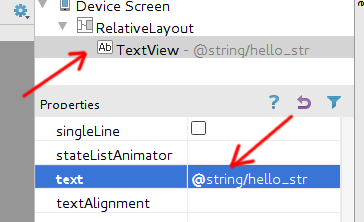
\includegraphics[scale=0.4]{chapters/ch04/images/8}
\end{center}

\texttt{\underline{Quick Exercise:}} Try changing the text of the text view to our new string resource with name \texttt{new\_Lbl}. Verify that it updates the app outlook properly. \\

\textbf{\underline{NEVER EVER} hardcode a string in your layouts that the user can potentially see}. The reason is that when using string ids in the xml code, if you want to change the language of your app then you just need to replace the \texttt{strings.xml} file with a different \texttt{strings.xml} containing different language strings (same name ids but different text). Your source code will remain EXACTLY the same and you won't have to change even a single line of code !!! \\

\textbf{\underline{WARNING:}} If you ever hardcode strings in your layouts, I'll haunt you in your dreams !!! \\

You can find detailed information about the string resource \href{https://developer.android.com/guide/topics/resources/string-resource.html}{here}.

\subsection{Supporting Multiple Languages}
The general concept is pretty simple. Our app will use string resource ids in the code. Whenever the app needs to display another language, it will \underline{automatically} switch the ``\texttt{strings.xml}'' with another appropriate one!

How does it actually do that? Well if the current language is ``English'', it will load the \texttt{strings.xml} from \texttt{values} directory. But if user selects say french from the phone settings then android OS will automatically load the \texttt{strings.xml} from \texttt{values-fr} directory. Note the suffix ``\texttt{-fr}'', it means french. \texttt{values-ur} is for urdu, \texttt{values-ar} is for arabic and so on. Each of these directories contains \texttt{strings.xml} files having strings of exactly same ids but different texts.

Let's add another language support. Open up the ``translation editor'' and click on the world icon located in the upper left corner of the editor. A huge list of available languages will appear in the drop down list. Select ``French (fr)'':

\begin{center}
	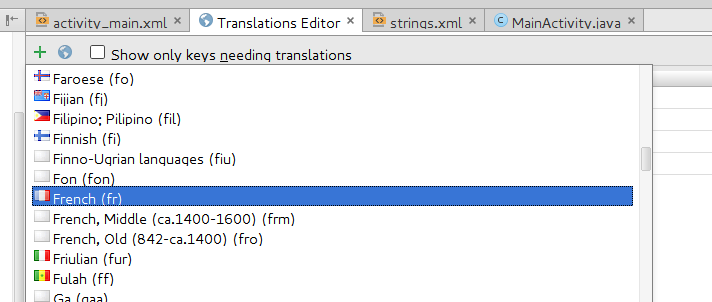
\includegraphics[scale=0.4]{chapters/ch04/images/16}
\end{center}

The translation editor will update itself to include french language. You can now add the french alternatives of the default text \textit{(and yes you need to go to \href{https://www.google.com/search?q=google+translate&ie=utf-8&oe=utf-8}{google translate} and add the translations here manually. Android studio won't magically translate stuff for you!)}. Also add urdu language:

\begin{center}
	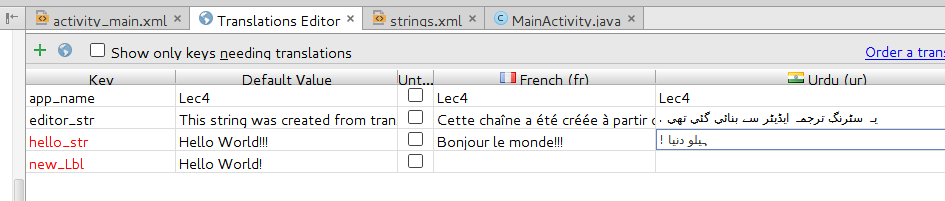
\includegraphics[scale=0.4]{chapters/ch04/images/17}
\end{center}

If you go to the project panel at the left side and analyze project directory structure, you'll notice that two new folders have been created to accommodate the new languages i.e: \texttt{values-fr} and \texttt{values-ur}. Each of these folders inturn contain \texttt{strings.xml}. Open these up and see what's inside:

\begin{center}
	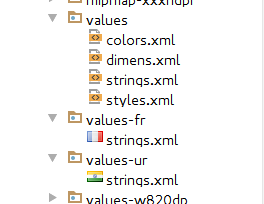
\includegraphics[scale=0.4]{chapters/ch04/images/18}
\end{center}

Make sure that the id of the text view is set to \texttt{@string/hello\_str}. Open up \texttt{activity\_main.xml} in design mode. Click on the earth icon located at the upper edge of the preview window, and select any of the available languages that we just added in the previous steps:

\begin{center}
	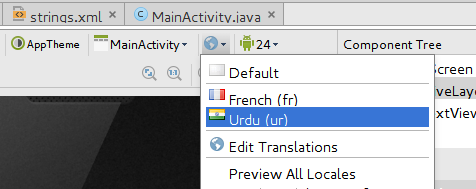
\includegraphics[scale=0.4]{chapters/ch04/images/19}
\end{center}

The preview should update to reflect new languages:

\begin{center}
	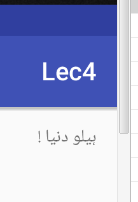
\includegraphics[scale=0.4]{chapters/ch04/images/20}
\end{center}

Also run the app on an emulator or actual phone. Go to your phone settings $\rightarrow$ Language and input $\rightarrow$ Language $\rightarrow$ Francais(France). Now run your app again and you should see following output:

\begin{center}
	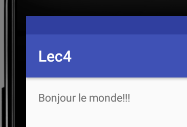
\includegraphics[scale=0.4]{chapters/ch04/images/21}
\end{center}

\vskip 3mm
You can visit \href{https://developer.android.com/training/basics/supporting-devices/languages.html}{this} link for more information on supporting multiple languages.

\subsection{Supporting Multiple Orientations}

Suppose that you made an app and it is looking great when in portrait mode. All of buttons and labels appear exactly where you want them to:

\begin{center}
	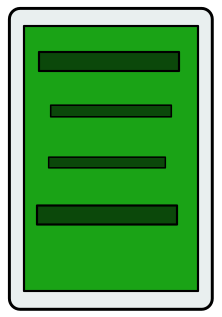
\includegraphics[scale=0.4]{chapters/ch04/images/22}
\end{center}

Now you switch your phone's orientation to landscape, if you have not designed your layout carefully then it will possibly stretch to account for the new screen size (eg: the \texttt{match\_parent} attribute was set). This stretching can potentially destroy all the aesthetics of your app and make it look hideous:

\begin{center}
	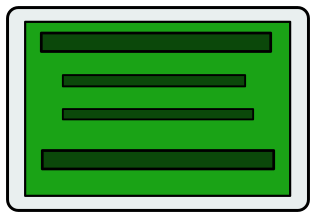
\includegraphics[scale=0.4]{chapters/ch04/images/23}
\end{center}

But if you were careful enough to design your layout so that they do not stretch with the new screen size, then you've got another problem. All of your controls will move to one side of the screen exposing ugly empty space where you could've put extra content:

\begin{center}
	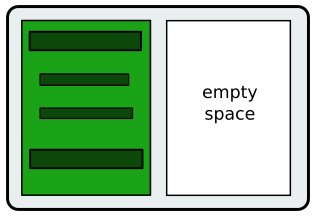
\includegraphics[scale=0.4]{chapters/ch04/images/24}
\end{center}

There is a solution to this problem! Just like when switching to a different language android studio automatically selects the appropriate \texttt{strings.xml} from multiple ones. When switching phone orientations android studio will \textbf{automatically} load the appropriate layout file from multiple ones. \\

\textit{``This means that we need to create multiple layout files having exact same name but possibly completely different content.''} \\

Open up \texttt{activity\_main.xml} in the design mode. Click on the ``Configuration to render this layout'' button located at the top left corner of the preview panel. Then select ``Landscape version'':

\begin{center}
	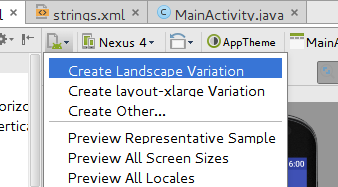
\includegraphics[scale=0.4]{chapters/ch04/images/25}
\end{center}

This will create a new folder called \texttt{``layout-land''} with a new file named {``activity\_main.xml'}' inside it. You can verify this from the project panel on the left side. When ever the phone is in landscape mode the app will automatically load this layout:

\begin{center}
	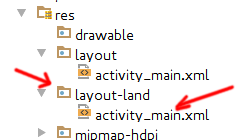
\includegraphics[scale=0.4]{chapters/ch04/images/26}
\end{center}

Now with your \texttt{activity\_main.xml} opened, make sure the orientation is switched to the landscape in the design mode. This will automatically load the correct layout xml file. Try to make a layout as shown below:

\begin{center}
	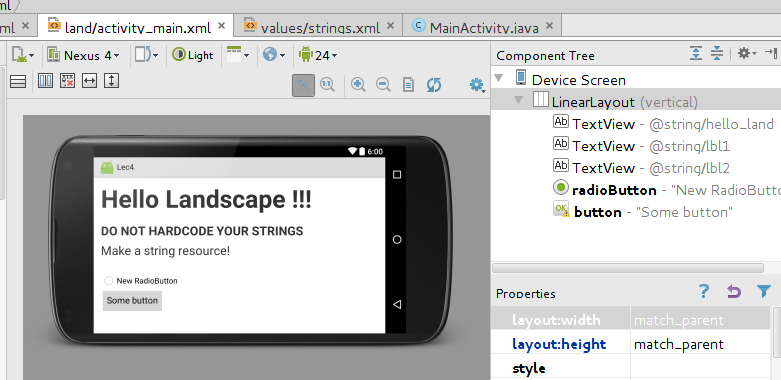
\includegraphics[scale=0.4]{chapters/ch04/images/27}
\end{center}

Now try switching the orientation and see if the correct layout is loaded. Also test this on emulator or the physical device. \\

For more information on supporting multiple orientations please visit: \href{https://developer.android.com/training/multiscreen/screensizes.html}{\textit{Supporting multiple screen sizes}}.

\section{Interactivity}
Before we begin to start coding we need some important concepts, one of which is the resource file.

\subsection{The ``\textbf{\texttt{R}}'' resource file}

Open up \texttt{activity\_main.xml} and go to design mode, make sure it's in portrait mode. Add a button and change it's \texttt{id} to ``\texttt{btn\_click}''. Change the button \textit{text} to ``Click me !!!'' (and you should make a string resource for it):

\begin{center}
	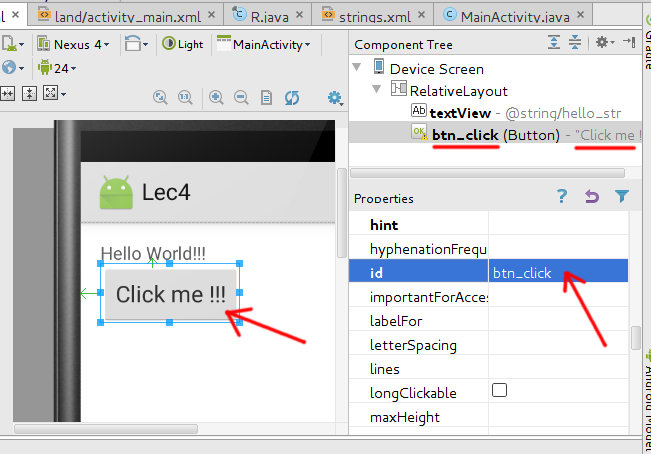
\includegraphics[scale=0.4]{chapters/ch04/images/30}
\end{center}

\textbf{Note:} Text string is completely different from \texttt{id}. The text is what you see displayed on a view. The \texttt{id} is a unique identifier that you will use to refer to the resources and views. Unlike text the \texttt{id} is not visible on the screen, it is used for internal book keeping and referencing resources. \\

Also change the \texttt{id} (NOT the text) of the text view label to ``\texttt{lbl\_hello}''. A dialog box will appear giving a warning to make changes. Click on yes:

\begin{center}
	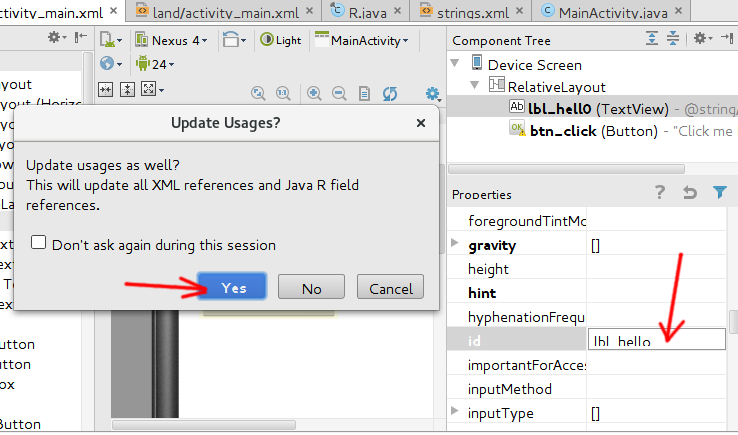
\includegraphics[scale=0.4]{chapters/ch04/images/31}
\end{center}

\textbf{Tip}: To specify an id just use a string literal, \textit{DO} NOT use a string resource like we used for the text field. \\

Double tap the \texttt{shift} key to open ``Search Everywhere'' dialog. Type ``\texttt{R}''. Two \texttt{R} class files will show up. Double click the one having the same package name as your project. Press \texttt{escape} key to dismiss the search pop-up if it is already there on the screen:

\begin{center}
	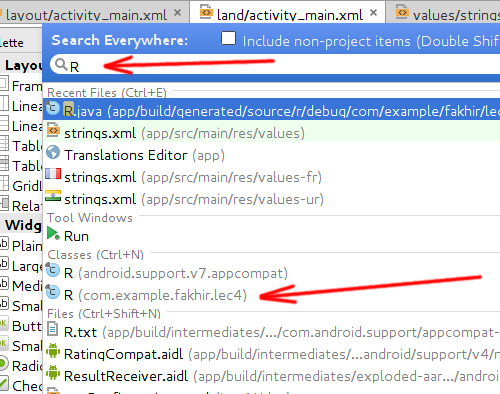
\includegraphics[scale=0.4]{chapters/ch04/images/28}
\end{center}

A java file named ``\texttt{R.java}'' will open up in the editor window. This is a very special class automatically generated by android studio. You must NEVER edit it manually (there is even a warning about this shown at the top of the file):

\begin{center}
	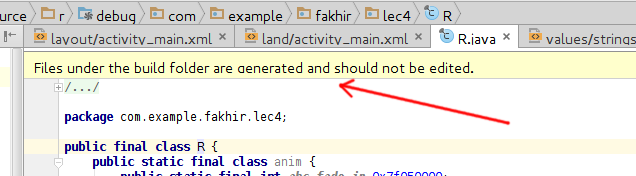
\includegraphics[scale=0.4]{chapters/ch04/images/29}
\end{center}

In android every view and every resource has an \texttt{id} assigned to it. The ``\texttt{R.java}'' file contains all the ids of every single thing in your app. There are many inner classes defined inside this file such as \texttt{anim}, \texttt{color}, \texttt{dimen} etc. Each of these contain constant integer member variables. \\

Let's find our button in ``\texttt{R.java}''. Search for ``\texttt{btn\_click}''. Well what do you know! It is just an integer member variable defined in the inner class \texttt{id} and assigned a ``unique'' integer number. We can access this button in the java code as ``\texttt{R.id.btn\_click}'' (line numbers in your case may differ):

\begin{center}
	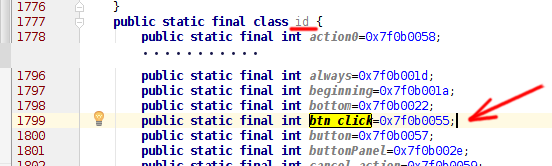
\includegraphics[scale=0.4]{chapters/ch04/images/32}
\end{center}

Apart from the button, our text view id is also contained inside the \texttt{id} inner class so we can access it as ``\texttt{R.id.lbl\_hello}''. In fact all of the view and view group ids are located under the \texttt{id} inner class.

Do we have string resource ids in here as well? Let's check. Search for any string resource ``name'' that we created earlier such as \texttt{hello\_str}. It is located under the ``\texttt{string}'' inner class. We can access this particular string recourse from our code as ``\texttt{R.}\textbf{\texttt{string}}\texttt{.hello\_str}''. You can also see the ids of other string resources that we created earlier. 

\begin{center}
	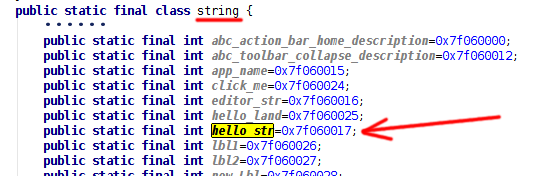
\includegraphics[scale=0.4]{chapters/ch04/images/33}
\end{center}

Other resources such as animations, pictures, sounds etc have their ids located under related inner classes.

\vskip 3mm
\textit{To summarize: Whatever id you assign to a view or a resource, it will automatically be converted into an integer member variable inside the ``\texttt{R}'' class and will be assigned a unique integer that you can use later on.}

\subsection{The inflator}
Remember an activity is made up of one or many layouts and exactly one java code file. Let's explore the code in our case. Since our project contains only one activity, there is only one java file. Open up \texttt{MainActivity.java} which is linked to the main activity. 

\begin{center}
	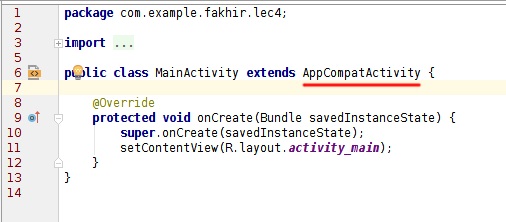
\includegraphics[scale=0.4]{chapters/ch04/images/34}
\end{center}

\texttt{MainActivity} class manages all the logic for this particular activity. Every activity class inherits the \texttt{Activity} class which contains essential code for running an activity. The first thing to notice in the above code is that \texttt{MainActivity} inherits \texttt{AppCompatActivity} class. \texttt{AppCompatActivity} basically extends \texttt{Activity} class to provide necessary support for action bar on older devices. You can find out more information about the \texttt{Activity} class \href{https://developer.android.com/reference/android/app/Activity.html}{here} and info about \texttt{AppCompatActivity} \href{https://developer.android.com/reference/android/support/v7/app/AppCompatActivity.html}{here}. \\

On line 9 there is a method called \texttt{onCreate}. Notice that this is a virtual function and it needs to be overridden (like its done above). When ever your activity is launched \texttt{onCreate} method is the first one to be called. For now ignore its parameters.

Line 10 is calling the \texttt{onCreate} for base class. Normally you don't have to modify this line.

Line 11 The \texttt{setContentView} method is something called an ``\textbf{inflator}''. An inflator basically takes an xml description of a layout and instantiates actual java objects that you see on the screen. Here it is taking \texttt{R.layout.activity\_main} and parses ``\texttt{activity\_main.xml}'' from the ``\texttt{layout}'' folder. When the device orientation is changed the activity is restarted and \texttt{onCreate} method is called. But this time depending on the orientation the inflator will automatically choose \texttt{activity\_main.xml} from ``\texttt{layout-land}'' folder and inflates a layout according to that. 

More information on layout inflators can be found \href{https://developer.android.com/reference/android/view/LayoutInflater.html}{here} and \href{http://stackoverflow.com/questions/2335813/how-to-inflate-one-view-with-a-layout}{here}. \\

Let's quickly create a new layout file. Select the ``Android'' mode from the project panel. Find the ``layout'' group and right click on it:

\begin{center}
	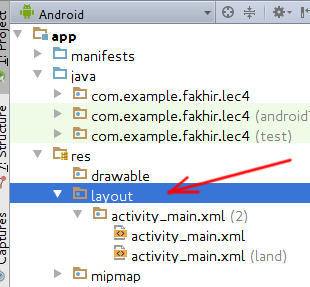
\includegraphics[scale=0.4]{chapters/ch04/images/39}
\end{center}

From the pop-up menu select ``New $\rightarrow$ Layout Resource file''. A dialog box will appear. Enter any name you want, say ``my\_text\_layout''. You can also specify the root element of the layout. When you create a new project the default root is the relative layout. But in this case the default is the linear layout, exactly what we want. For other fields accept the defaults and hit OK:

\begin{center}
	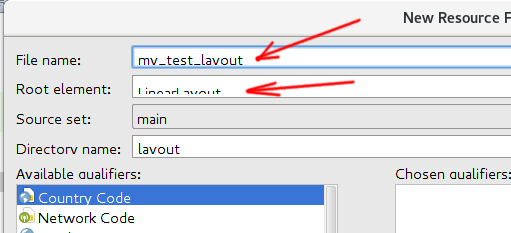
\includegraphics[scale=0.4]{chapters/ch04/images/40}
\end{center}

Now a new layout file named ``\texttt{my\_test\_layout.xml}'' should be created in your project directory. Open it up and create any simple layout that you want, such as following:

\begin{center}
	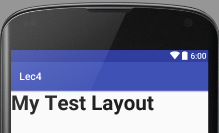
\includegraphics[scale=0.4]{chapters/ch04/images/41}
\end{center}

We've created a new layout. We can now refer it in our code as ``\texttt{R.layout.my\_test\_layout}''. Go back to \texttt{MainActivity.java} and modify the line 12 as follows:

\begin{center}
	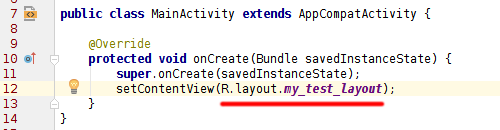
\includegraphics[scale=0.4]{chapters/ch04/images/42}
\end{center}

The \texttt{setContentView} inflator function will parse our new xml and inflate a totally new layout on the screen. Run the app to see the changes on the device:

\begin{center}
	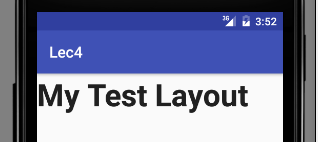
\includegraphics[scale=0.4]{chapters/ch04/images/43}
\end{center}

Great, this tells us that we can use ANY layout file that we want anywhere we want and whenever we want with any activity we want! \\

\underline{\textbf{Important:}} Now undo the changes you've just made and modify line 12 back to the following:

\texttt{setContentView(R.layout.activity\_main);}

because the next sections are relying on that.


\subsection{Output Log}
You can print different log messages to the dedicated console window. This is extremely useful for debugging. Inside the \texttt{onCreate} method add the code shown in line 14 below:

\begin{center}
	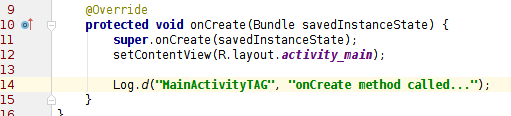
\includegraphics[scale=0.4]{chapters/ch04/images/35}
\end{center}

As you start typing the keywords android studio will try to auto-complete and show you a pop-up of multiple options to select from. Choose \texttt{Log.d}. The \texttt{d} stands for debug output. You can use \texttt{Log.e} to print an error. 

\texttt{Log.d} takes two parameters. The first one is something called a TAG. TAG  is used to identify the source of a log message, so we named it ``\texttt{MainActivityTAG}'' here. The second parameter is the actual message that you want to print on the console.

Run the app on emulator or the device. You should see the android monitor panel appeared on the bottom side of the screen. If not then click ``Android Monitor'' tab located at the very bottom edge of the screen:

\begin{center}
	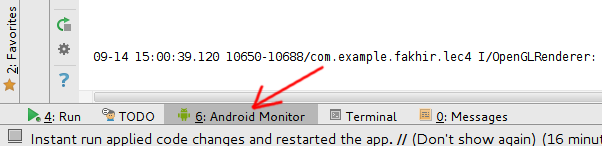
\includegraphics[scale=0.4]{chapters/ch04/images/36}
\end{center}

Make sure that the ``Logcat'' tab is selected. Also make sure that you've selected the correct device and also the correct package related to this particular app:

\begin{center}
	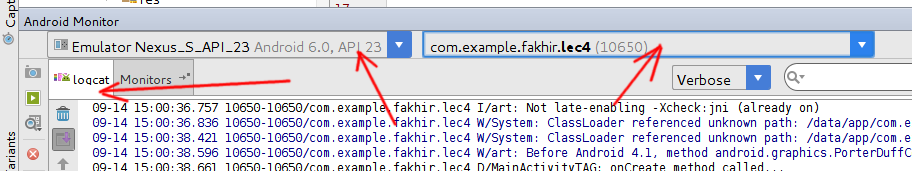
\includegraphics[scale=0.4]{chapters/ch04/images/37}
\end{center}

The android monitor window shows all sorts of messages being dumped on the screen. It is really hard to find our log message that we displayed from all of this huge pile. Go back to the activity monitor and make sure that the ``verbose'' mode is selected and also ``Show only selected application'' is selected from the drop down menu at the right (shown below). Remember the TAG string we gave in \texttt{Log.d}? As you type the TAG in the search field, only the related messages will filter out and you'll see just a handful of messages on the console:

\begin{center}
	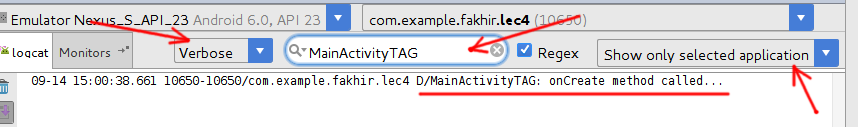
\includegraphics[scale=0.4]{chapters/ch04/images/38}
\end{center}

Find out more about the logging \href{https://developer.android.com/reference/android/util/Log.html}{here}. \\

\subsection{Getting View Reference}
You can get the reference to any view via it's \texttt{id}. Remember that after inflating the views become java object at run-time. There is a method called \underline{``\texttt{findViewById}''} which takes the id of a view as argument and returns reference to the view object in memory. 

More information about \texttt{findViewById} is given \href{https://developer.android.com/reference/android/view/View.html}{here}. \\

\subsection{Changing View attributes dynamically}
Let's change the text of our button and the text view label present on out \texttt{activity\_main.xml} layout (portrait mode). Remember that we set the view ids as follows:

\begin{center}
	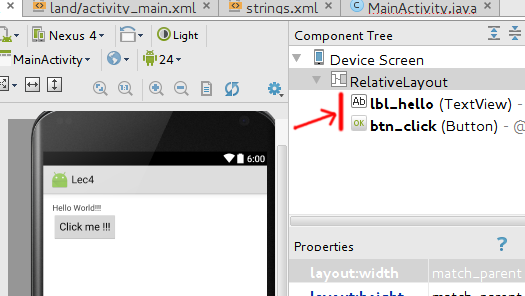
\includegraphics[scale=0.4]{chapters/ch04/images/44}
\end{center}

Open up \texttt{MainActivity.java} and inside the \texttt{onCreate} method add the following lines:

\begin{center}
	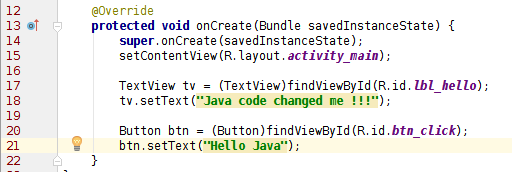
\includegraphics[scale=0.4]{chapters/ch04/images/45}
\end{center}

Also remember that the ids of the views are stored in the \texttt{id} inner class inside the \texttt{R} class. Line 17 is accessing the id of our text label as \texttt{R.id.lbl\_hello} and passing it as argument to the ``\texttt{findViewById}'' method. Then \texttt{findViewById} returns a \texttt{View} object which needs to be casted into \texttt{TextView} type and then finally stored in the reference variable named \texttt{tv}.

Line 18 is then accessing the attributes for this particular and setting it through code. Here we are setting the text of the label. You can set ANY attribute imaginable through this method.

Lines 20 and 21 are getting reference to the button and changing its text. When you run the app you will see the following output:

\begin{center}
	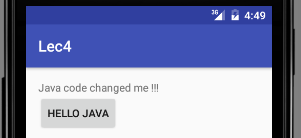
\includegraphics[scale=0.4]{chapters/ch04/images/46}
\end{center}

Alternatively, instead of giving hard-coded string literals you can specify the string resource ids to set the text for any view (line 18):

\begin{center}
	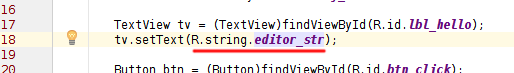
\includegraphics[scale=0.4]{chapters/ch04/images/47}
\end{center}

\subsection{Interacting with the Views}
Bunch of pretty buttons on the screen is no good if they do anything. Whenever a user interacts with a view an event is generated. Whenever an even is generated a special function known an event handler is called (more information about the concept of events and event handlers can be found \href{https://en.wikipedia.org/wiki/Event_(computing)}{here}). 

The event handlers in android must have the following signature:

\begin{verbatim}
public void MethodName(View view) {
    ...
}
\end{verbatim}

It must be a public method having return type \texttt{void}. It must have exactly one parameter of type \texttt{View}. This represents the view object that called this event handler. 

Let's add an event handler for our button using the simplest possible method. We will see other methods in future lectures. \\

Open up \texttt{activity\_main.xml} (portrait mode) and switch to the text mode. Inside the \texttt{<Button>} tag add an \texttt{onClick} attribute and assign it any name such as \texttt{onBtnClickFn} (line number 26 shown below):

\begin{center}
	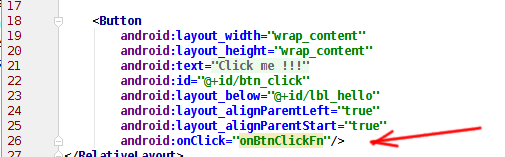
\includegraphics[scale=0.4]{chapters/ch04/images/48}
\end{center}

Bring the keyboard cursor on the \texttt{onBtnClickFn} string literal. A yellow bulb will appear on the left side. Click it and select ``Create in `onBtnClickFn(View)' MainActivity'':

\begin{center}
	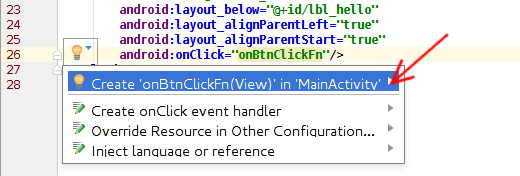
\includegraphics[scale=0.4]{chapters/ch04/images/49}
\end{center}

This will automatically create an event handler method and link it to the button. Go to \texttt{MainActivity.java} and you'll see the method created in the \texttt{MainActivity} class. Whenever you click the button this method will be executed:

\begin{center}
	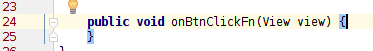
\includegraphics[scale=0.4]{chapters/ch04/images/50}
\end{center}

\subsection{Controlling views from other views}

Let's change the label text whenever our button is clicked. Open up \texttt{MainActivity.java} and go to our newly created event handler method \texttt{onBtnClickFn}. Add the following lines:

\begin{center}
	\includegraphics[scale=0.4]{chapters/ch04/images/51}
\end{center}

Line 25 gets the reference to the text view object. 

Line 26 sets the desired text whenever the button is clicked. \\

Run the app, click the button and see if the text is changed:

\begin{center}
	\includegraphics[scale=0.4]{chapters/ch04/images/52}
\end{center}

\section{Exercise: Tip calculator}

Create an app that calculates tip to be paid using simple information entered through edit text fields:

\begin{center}
	\includegraphics[scale=0.4]{chapters/ch04/images/53}
\end{center}

\subsection{Solution:}
\underline{\textbf{Warning}}: The next page contains the solution to this exercise. Try it yourself first before viewing the solution.

\newpage
Only the event listener function and logic is shown (you can appropriately set the id's of the views in the layout file yourself):
\begin{center}
	\includegraphics[scale=0.4]{chapters/ch04/images/54}
\end{center}
